        \clearpage
        \begin{figure*}[ht]
            \pdfbookmark[2]{ID 06}{figure_id_06}
        	\centering
            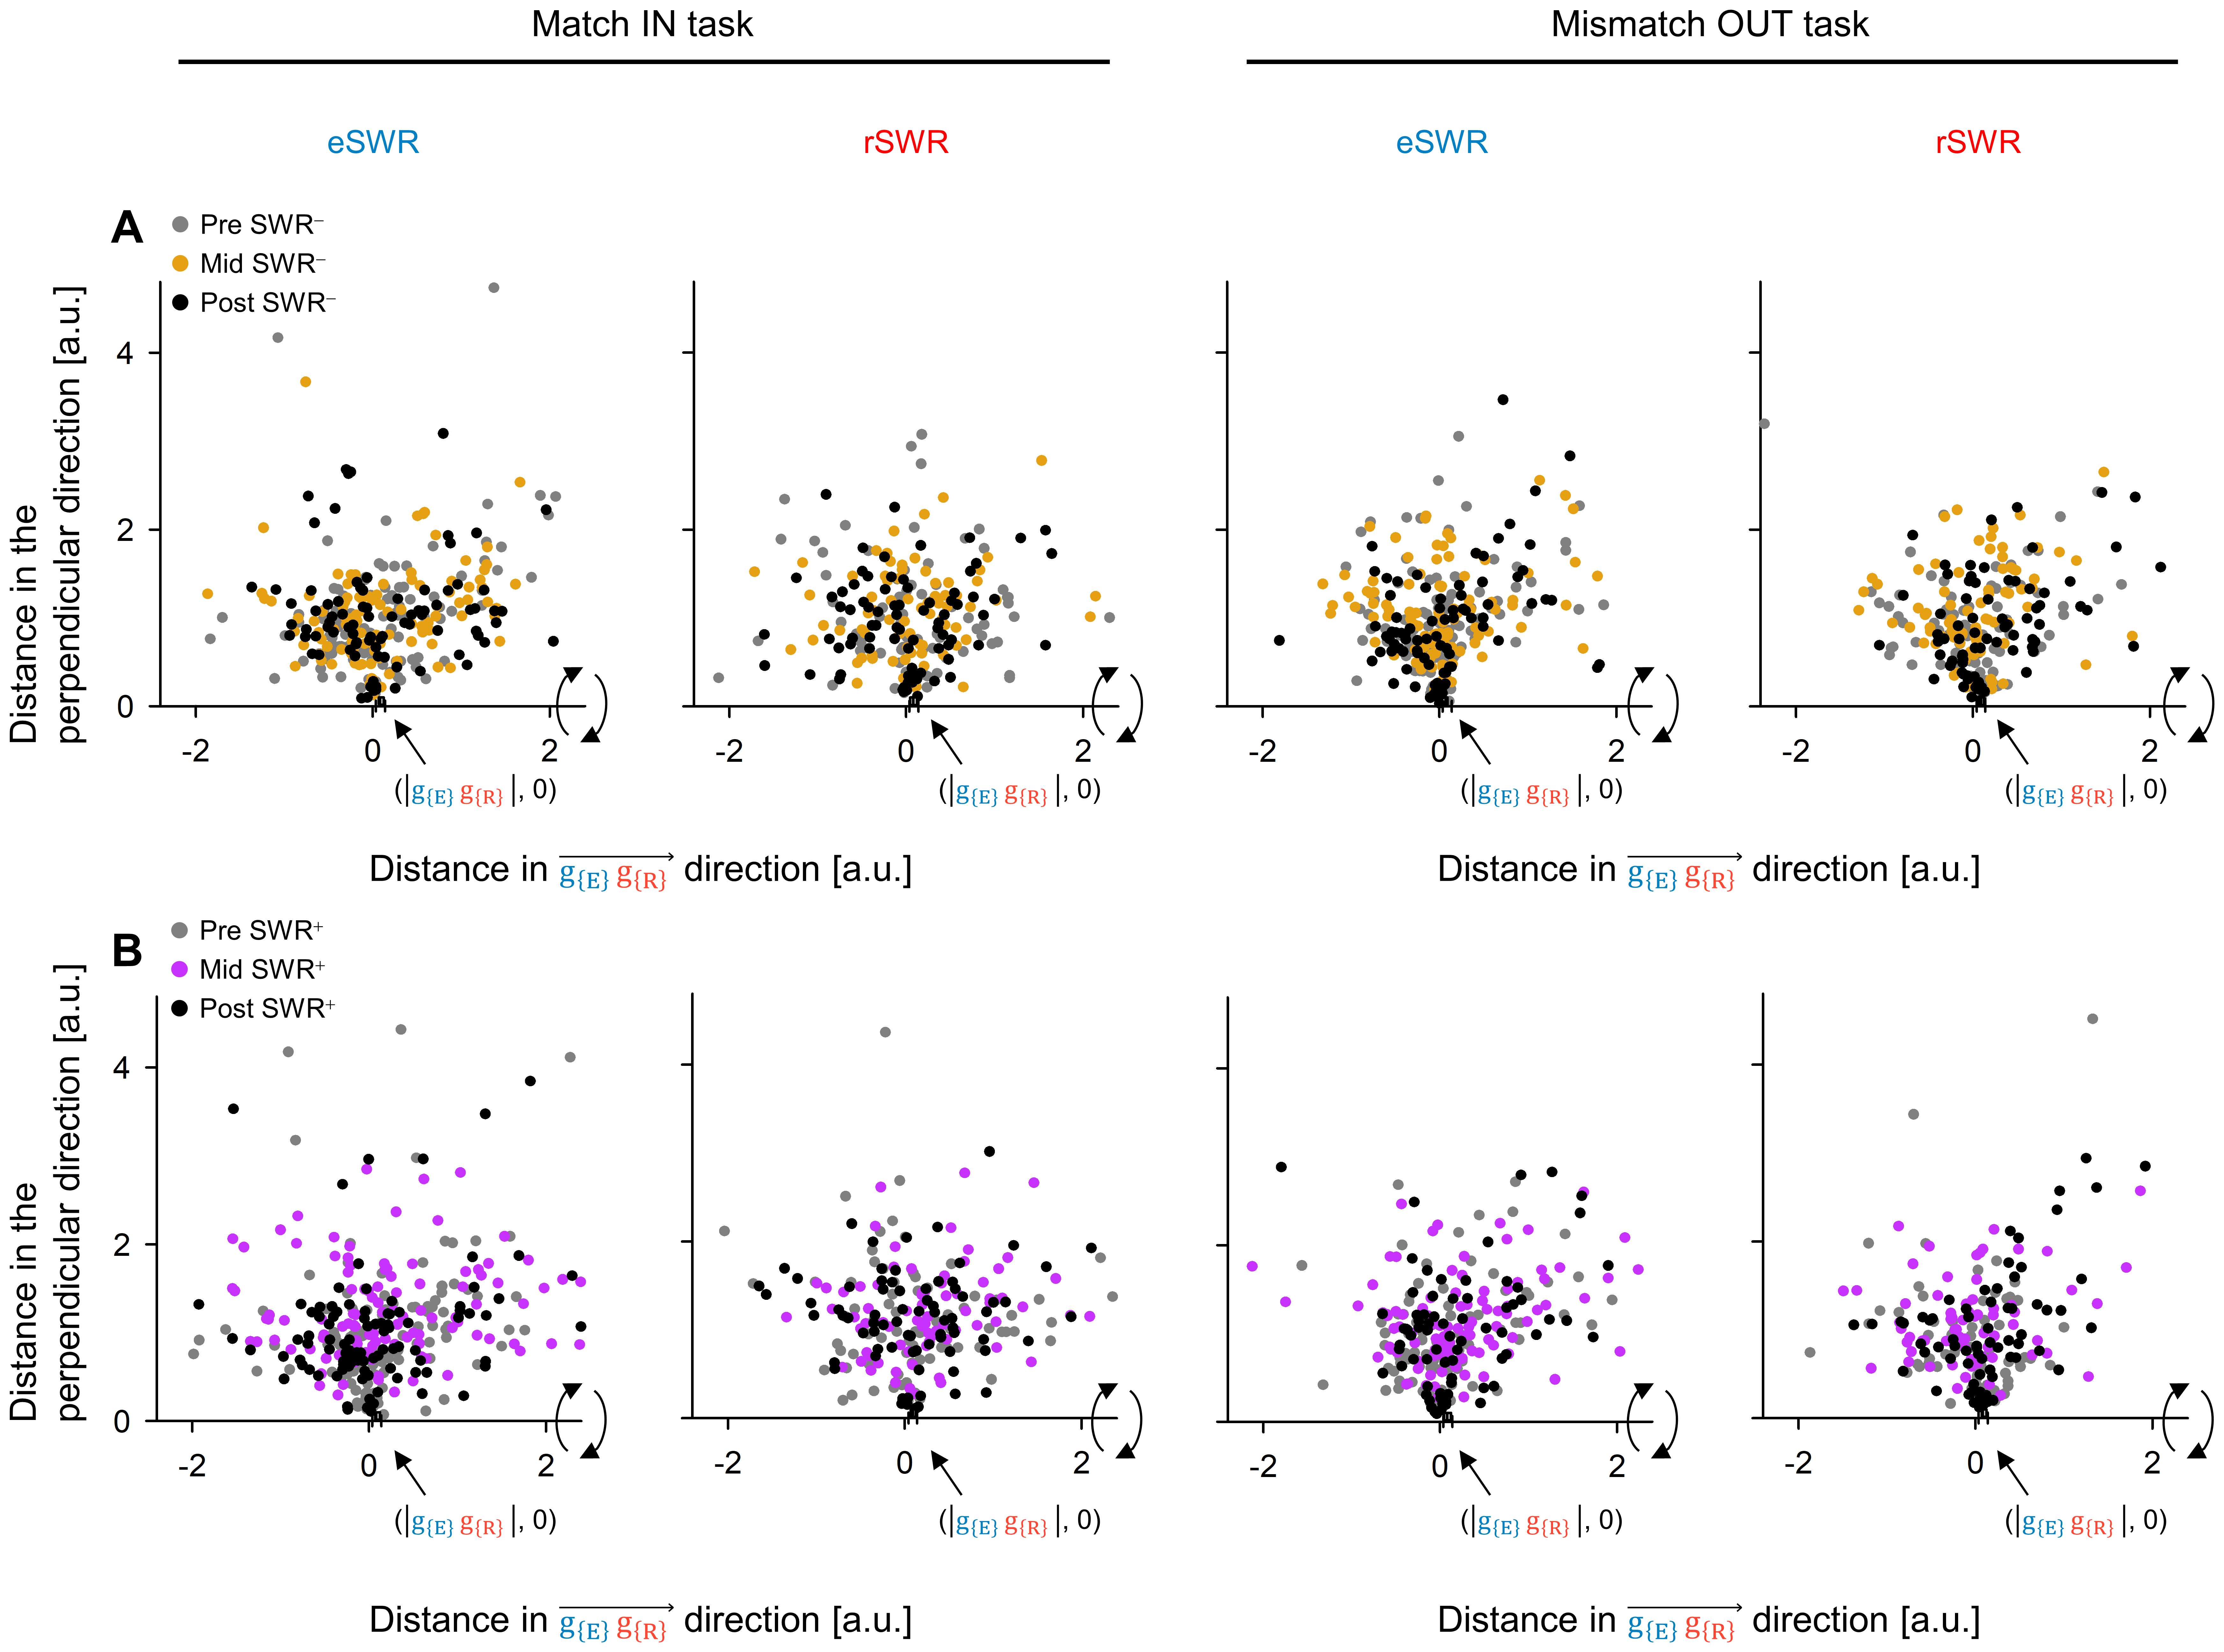
\includegraphics[width=1\textwidth]{./src/figures/.png/Figure_ID_06.png}
        	\caption{\textbf{
Visualization of Neural Trajectory During SWR in Two-Dimensional Space
}
\smallskip
\\
Featured are neural trajectories within the hippocampus during Sharp-Wave Ripple (SWR) events, represented in a two-dimensional space. \textbf{\textit{A.}} Trajectories during pre- (\textit{gray}), mid- (\textit{yellow}), and post-SWR$^-$ (\textit{black}) phases of an SWR event~\cite{buzsaki_hippocampal_2015}. \textbf{\textit{B.}} Corresponding trajectories for SWR$^+$ scenarios as opposed to SWR$^-$~\cite{fernandez-ruiz_long-duration_2019}. The magnitude of $\lVert \mathrm{g_{E}g_{R}} \rVert$ fluctuates within sessions~\cite{liu_consensus_2022}. The projection protocol went as follows: initially, $\mathrm{g_{E}}$ was placed at the origin $O$ (0,0), and $\mathrm{g_{R}}$ at ($\lVert \mathrm{g_{E}g_{R}} \rVert$, 0) via linear transformation~\cite{kim_corticalhippocampal_2022}. Subsequently, the point cloud was rotated around the $\mathrm{g_{E}g_{R}}$ axis (the x-axis) for compatibility with a two-dimensional environment~\cite{yu_gaussian-process_2009}. Consequently, both the distances from $O$ and the angles with respect to the $\mathrm{g_{E}g_{R}}$ axis were kept intact from their original three-dimensional arrangement~\cite{mcinnes_umap_2018}. Abbreviations: SWR denotes Sharp-Wave Ripple events; eSWR refers to SWR during the encoding phase; rSWR indicates SWR during the retrieval phase; SWR$^+$ represents an SWR event; SWR$^-$ designates the control events for SWR$^+$; pre-SWR, mid-SWR, or post-SWR specify the time interval from $-800$ to $-250$ ms, from $-250$ to $+250$ ms, or from $+250$ to $+800$ ms from the center of the SWR respectively~\cite{zhang_hippocampal_2022}.
}
% width=1\textwidth
        	\label{fig:06}
        \end{figure*}
